\subsection{Classification des syndromes aphasique}

La définition que nous avons donnée de l'aphasie s'applique à une multitude de troubles
(ou \emph{syndromes}) dissimilaires en causes (région touchée du cerveau) 
et effets (conséquences pour la communication)~\cite{Hallowell_2017}.
La table~\ref{tab.aphasia-classification} 
et la figure~\ref{fig.aphasia-tree}
présentent une classification des syndromes aphasiques classiques.
\begin{table}[ht]
    \centering
    \begin{adjustbox}{max width=15cm}
        \begin{tabular}{|p{3cm}|p{3cm}|p{3cm}|p{3cm}|p{3cm}|}
        \hline
        Syndrome Aphasique                                      & 
        Expressive / Réceptive                                  & 
        Localisation de la Lésion                               & 
        Effet sur la Compréhension                              & 
        Effet sur l'Expression                                  \\
        \hline
        Aphasie de Wernicke                                     & 
        Réceptive                                               & 
        Aire de Wernicke (Brodmann 22 \footcite{Brodmann_2007}) &
        Modéré à sévère                                         & 
        Modéré à sévère                                         \\
        \hline
        Aphasie de Broca                                        &
        Expressive                                              &
        Aire de Broca (Brodmann 44, 45)                         &
        Léger à modéré                                          &
        Modéré à sévère                                         \\
        \hline
        Aphasie de Conduction                                   &
        Les deux                                                &
        Brodmann 40                                             &
        Léger à modéré                                          &
        Léger à modéré                                          \\
        \hline
        Aphasie Globale                                         &
        Expressive                                              &
        Large, touche à plusieurs régions                       &
        Sévère                                                  &
        Sévère                                                  \\
        \hline
        Aphasie Transcorticale Sensorielle                      &
        Réceptive                                               &
        Brodmann 37, 39                                         &
        Modéré à sévère                                         &
        Modéré à sévère                                         \\
        \hline
        Aphasie Transcorticale Motrice                          &
        Expressive                                              &
        Brodmann 6, 8--10, 46                                   &
        Léger à modéré                                          &
        Léger à modéré                                          \\
        \hline
        Aphasie Transcorticale Mixte                            &
        Expressive                                              &
        Lobe Frontal inférieur                                  &
        Léger à modéré                                          &
        Léger à modéré                                          \\
        \hline
        \end{tabular}
    \end{adjustbox}
    \caption[Classification des syndromes aphasiques classiques.]%
    {Classification des syndromes aphasiques classiques~\cite{Hallowell_2017}}
    \label{tab.aphasia-classification}
\end{table}
\begin{figure}[htb]
    \begin{center}
        \resizebox{\textwidth}{!}{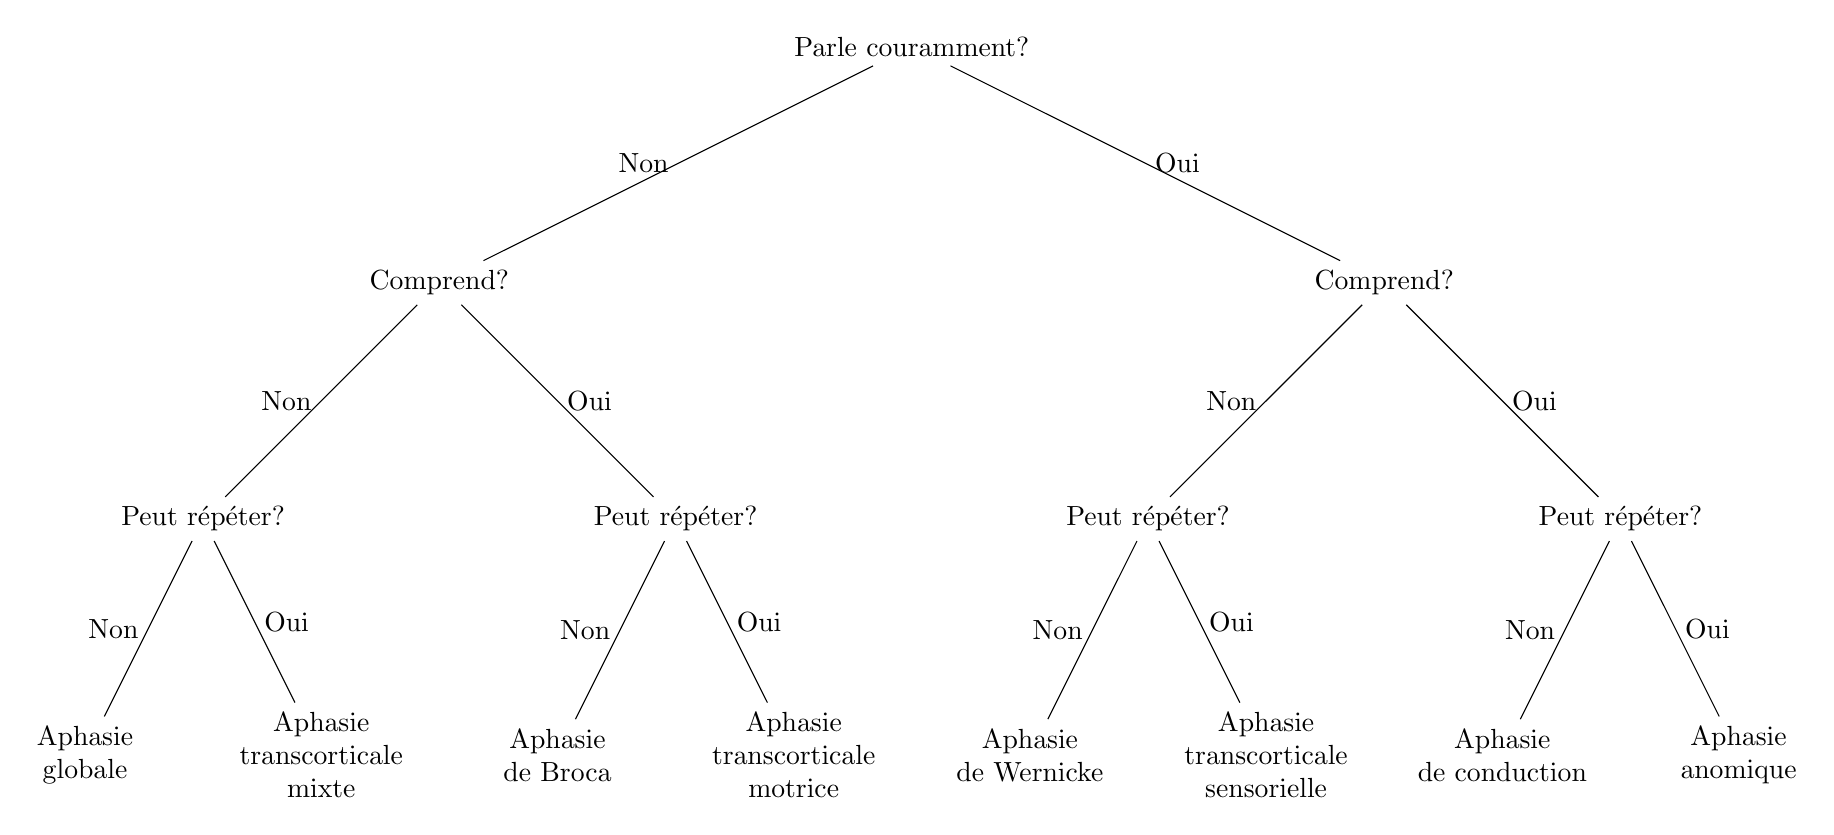
\begin{tikzpicture}
    [level distance=3cm,
    level 1/.style={sibling distance=12cm},
    level 2/.style={sibling distance=6cm},
    level 3/.style={sibling distance=3cm}
    ]
    \tikzstyle{bag} = [align=center]
    \tikzset{every tree node/.style={align=center,anchor=north}}
    % \tikzset{level distance=2cm, sibling distance=5cm}
    \node (Root)  {Parle couramment?}
        child {
            node {Comprend?} 
            child {
                node {Peut répéter?}
                child {node[bag] {Aphasie\\globale} edge from parent node[left] {Non }} 
                child {node[bag] {Aphasie\\transcorticale\\mixte} edge from parent node[right] {Oui }} 
                edge from parent node[left] {Non}   
            }
            child {
                node {Peut répéter?}
                child {node[bag] {Aphasie\\de Broca} edge from parent node[left] {Non }} 
                child {node[bag] {Aphasie\\transcorticale\\motrice} edge from parent node[right] {Oui }} 
                edge from parent node[right] {Oui}   
            } 
            edge from parent node[left] {Non} 
        }
        child {
            node {Comprend?} 
            child {
                node {Peut répéter?}
                child {node[bag] {Aphasie\\de Wernicke} edge from parent node[left] {Non }} 
                child {node[bag] {Aphasie\\transcorticale\\sensorielle} edge from parent node[right] {Oui }} 
                edge from parent node[left] {Non}   
            }
            child {
                node {Peut répéter?}
                child {node[bag] {Aphasie\\de conduction} edge from parent node[left] {Non }} 
                child {node[bag] {Aphasie\\anomique} edge from parent node[right] {Oui }} 
                edge from parent node[right] {Oui}   
            } 
            edge from parent node[right] {Oui} 
        };
    
    \end{tikzpicture}}
    \end{center}
    \caption[Classification des syndromes aphasiques classiques.]
    {Classification des syndromes aphasiques classiques~\cite{Sreedharan_2018}.}
    \label{fig.aphasia-tree}
\end{figure}
En particulier, notre sujet d'intérêt, l'aphasie de Broca, est une aphasie expressive.
Elle affecte surtout la production du langage.
Sa compréhension est généralement préservée.
De ce fait, les personnes atteintes de l'aphasie de Broca sont conscientes de leur handicap~\cite{Chapey_2008}.
